\FloatBarrier
\subsection{Central degradation curves and conditional contributions}
\label{sec:r43}
Figure~\ref{fig:r43-central} is the central end-to-end result: all four
actual configurations on two severity slices, holding $ p=p_{\rm ID}$ while
varying SNR and $ S=S_{\rm ID}$ while varying $ p $.
Eight SNR and 15 BSC conditions share one anchor point, hence 22 unique
conditions; this is not a full two-dimensional response surface.
The 1400 held-out bundles use disjoint phase-1 leaves:
\begin{equation}
 \text{Gaussian}: (1,4,1,s_G,r),\qquad
 \text{BSC}: (2,4,1,s,r,c),\quad r=0,\ldots,1399.
 \label{eq:r43-paths}
\end{equation}
There are \WPaths{} paths,\WGaussian{} unique Gaussian vectors and
 \WMasks{} positive-$ p $ masks. Reused inputs do not multiply independent
exposure. At $ p=0 $ Gaussian noise remains; 00=01 and 10=11 exactly.
Four no-Gaussian/$ p=0 $ controls run once outside the random means.

Approximate Bonferroni t/CLT intervals use 1400 complete bundles and the
prespecified 92-statistic family (Eq.~\eqref{eq:r43-mean-ci}); they are
mean intervals, not per-record spread or exact finite-sample guarantees.
The 12-condition main objective first averages each bundle's 12 equally
weighted, unique main conditions, then estimates uncertainty from 1400
bundle scores (Eq.~\eqref{eq:r43-main-objective}). Diagnostic/refinement
points have zero main weight; the personal overlap is counted once.
The weights are a design objective, not observed channel probabilities.

\begin{figure}[!htbp]
 \centering
 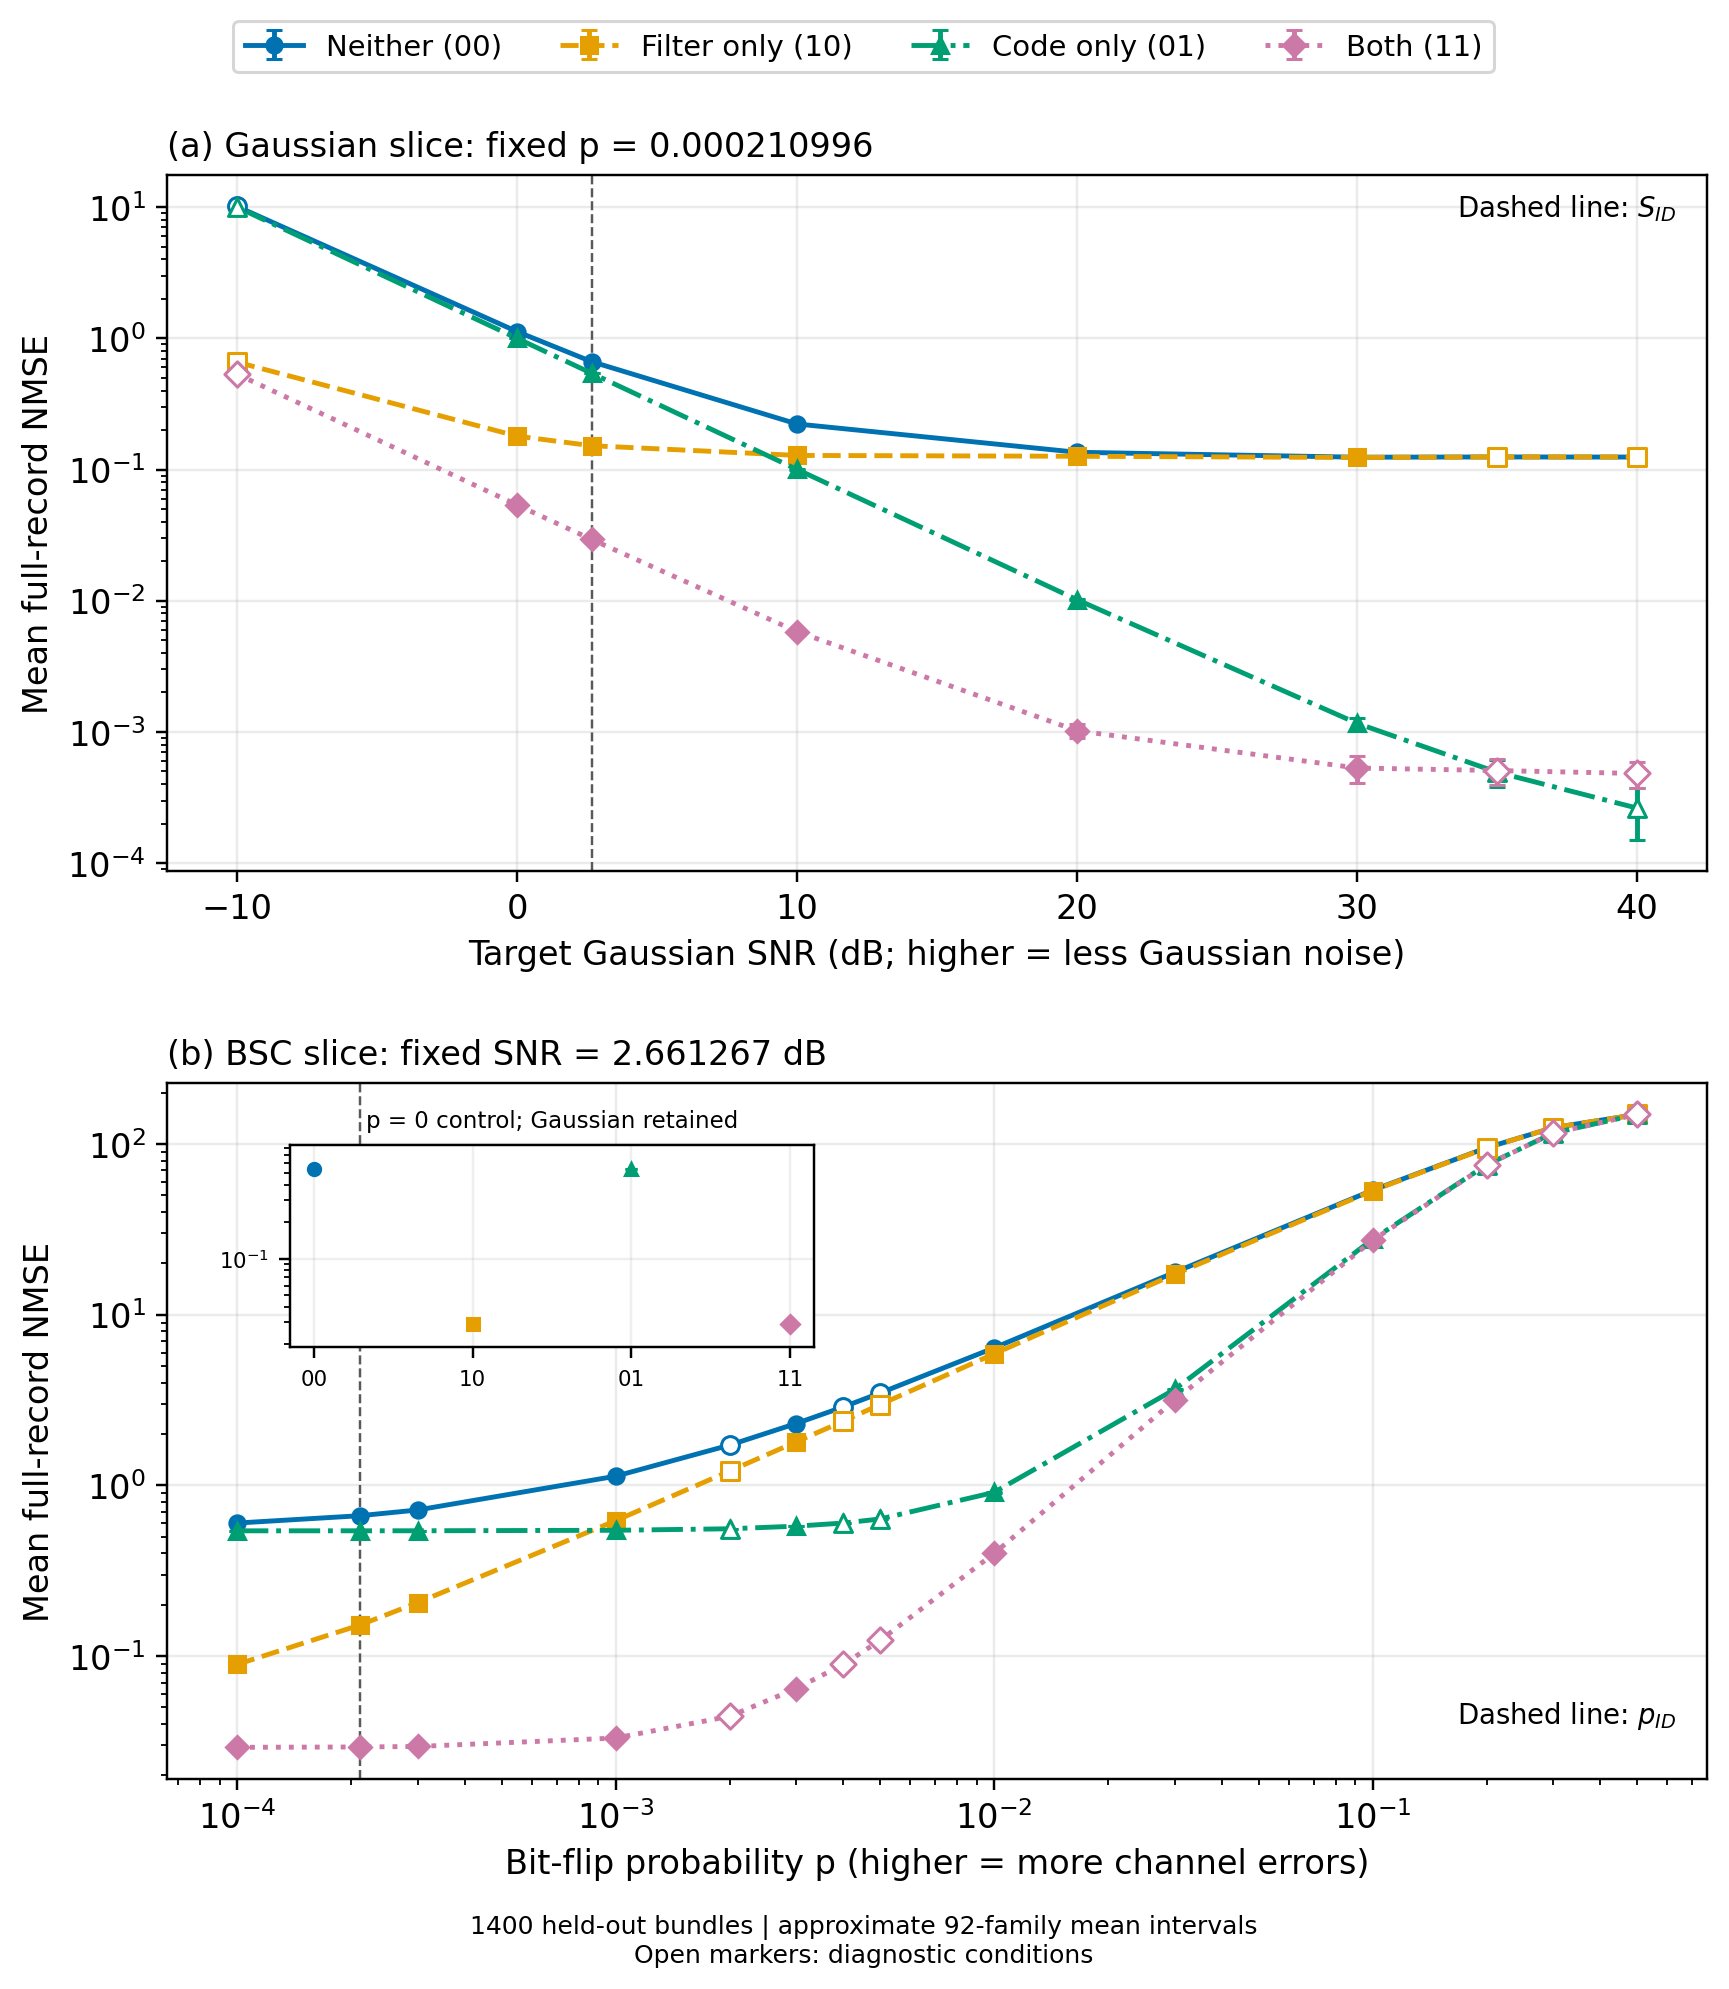
\includegraphics[width=.88\linewidth]{images/r43_central_quality.png}
 \caption{Four configurations, 1400 bundles, approximate 92-family mean intervals. Positive $p$: log axis; inset: $p=0$ with Gaussian retained. Filled/open: main/diagnostic points; lines join tested points only.}
 \label{fig:r43-central}
\end{figure}


\begin{table}[htbp]
 \centering\small
 \caption{Held-out anchor-point results. Only NMSE intervals belong to the 92-mean family; MAE and real-information BER are descriptive.}
 \label{tab:r43-personal}
 \begin{tabular}{lrrrr}
\toprule
Config. & Mean NMSE & Adjusted mean interval & Mean MAE & Data BER \\
\midrule
00 & 0.664309 & [0.660879, 0.667739] & 0.513143 & $2.1117\times10^{-4}$ \\
10 & 0.151933 & [0.148476, 0.155391] & 0.131631 & $2.1117\times10^{-4}$ \\
01 & 0.541989 & [0.541564, 0.542413] & 0.501820 & $3.7946\times10^{-7}$ \\
11 & 0.029339 & [0.029190, 0.029488] & 0.116303 & $3.7946\times10^{-7}$ \\
\bottomrule
\end{tabular}

 
 
\end{table}

% Keep the run-in heading and its complete result paragraph on the same page.
\noindent\begin{minipage}{\linewidth}
\paragraph{What the curves establish.}
At the anchor point, neither/filter-only/code-only/both mean NMSEs are
$\WPersonalNeither $, $\WPersonalFilter $, $\WPersonalCode $ and
$\WPersonalBoth $. Both gives the lowest error: coding alone leaves most
Gaussian error; filtering alone leaves unprotected bit corruption.
As SNR rises, the uncoded BSC floor persists. At 40 dB code-only/both means
are $\WHighCode/\WHighBoth $; the estimated filter reduction
$\WHighFilterReduction $ has conservative interval
$[\WHighFilterLower,\WHighFilterUpper]$, including zero.
The apparent reversal is therefore not established by the primary rule.
Separate clean controls do establish FIR distortion: NMSE
$\WCleanRaw $ without filtering and $\WCleanFilter $ with it.
\end{minipage}\par

\begin{table}[htbp]
 \centering\small
 \caption{Conditional NMSE reductions and interaction at the anchor/high-SNR points. Positive reductions improve quality; conservative intervals retain negative and unresolved effects.}
 \label{tab:r43-effects}
 \begin{tabular}{llrr}
\toprule
Condition & Contrast & Mean reduction & Conservative interval \\
\midrule
Personal & $G_{F\mid C=0}$ & $5.1238\times10^{-1}$ & $[5.0549\times10^{-1}, 5.1926\times10^{-1}]$ \\
Personal & $G_{F\mid C=1}$ & $5.1265\times10^{-1}$ & $[5.1208\times10^{-1}, 5.1322\times10^{-1}]$ \\
Personal & $G_{C\mid F=0}$ & $1.2232\times10^{-1}$ & $[1.1847\times10^{-1}, 1.2618\times10^{-1}]$ \\
Personal & $G_{C\mid F=1}$ & $1.2259\times10^{-1}$ & $[1.1899\times10^{-1}, 1.2620\times10^{-1}]$ \\
Personal & $I$ & $-2.7385\times10^{-4}$ & $[-7.7348\times10^{-3}, 7.1871\times10^{-3}]$ \\
40 dB & $G_{F\mid C=0}$ & $-2.1906\times10^{-4}$ & $[-7.1277\times10^{-3}, 6.6896\times10^{-3}]$ \\
40 dB & $G_{F\mid C=1}$ & $-2.1972\times10^{-4}$ & $[-4.4259\times10^{-4}, 3.1494\times10^{-6}]$ \\
40 dB & $G_{C\mid F=0}$ & $1.2422\times10^{-1}$ & $[1.2065\times10^{-1}, 1.2778\times10^{-1}]$ \\
40 dB & $G_{C\mid F=1}$ & $1.2422\times10^{-1}$ & $[1.2065\times10^{-1}, 1.2778\times10^{-1}]$ \\
40 dB & $I$ & $6.6129\times10^{-7}$ & $[-7.1309\times10^{-3}, 7.1322\times10^{-3}]$ \\
\bottomrule
\end{tabular}

 
 
\end{table}

The conditional contrasts above inherit conservative bounds from the
joint mean event (Appendix~\ref{app:statistics}); paired pointwise
intervals are separate exploratory results. Nonadditivity is retained.
At $ p=0.5 $ independently fair recovered labels predict NMSE 148.960954
for every configuration, and all four measured intervals contain it.
This is the random-label model of Appendix~\ref{app:quant}, not small
quantisation noise $\Delta^2/12 $.

\begin{table}[htbp]
 \centering\small
 \caption{Twelve-condition equal-weight objective from 1400 independent bundle scores. Intervals belong to the 92-statistic family; weights are design choices, not channel frequencies.}
 \label{tab:r43-objective}
 \begin{tabular}{lrrrr}
\toprule
Config. & $\bar J$ & Adjusted mean interval & Half-width (\%) & kbit/s \\
\midrule
00 & 7.06272 & [7.05624, 7.06919] & 0.09 & 224 \\
10 & 6.65633 & [6.64974, 6.66293] & 0.10 & 224 \\
01 & 3.00505 & [3.00105, 3.00905] & 0.13 & 392 \\
11 & 2.58806 & [2.58400, 2.59211] & 0.16 & 392 \\
\bottomrule
\end{tabular}

 
 
\end{table}

The objective summarises only its declared 12-condition domain.
Using Eq.~\eqref{eq:r43-contrast}, adjacent objective differences
$J_{00}-J_{10}$, $J_{10}-J_{01}$ and $J_{01}-J_{11}$ have conservative
outward-rounded intervals $[0.39331,0.41946]$, $[3.64069,3.66188]$ and
$[0.40893,0.42506]$, respectively. All are positive on the approximate
joint mean event, supporting $J_{11}<J_{01}<J_{10}<J_{00}$ for these
weights. This weighted-average ranking does not assert the same ordering
at every SNR/$p$, or in a different channel population.

\begin{table}[htbp]
 \centering\small
 \caption{Configuration 11 full-grid component powers, including small terms, plus signed cross terms. Sampling-scale residuals here are numerical, not measurable aliasing.}
 \label{tab:r43-components}
 \begin{tabular}{lrr}
\toprule
Term (configuration 11) & Personal point & 40 dB, personal $p$ \\
\midrule
Sampling & $1.7504\times10^{-25}$ & $1.7504\times10^{-25}$ \\
Filter & $2.2951\times10^{-4}$ & $2.2951\times10^{-4}$ \\
Gaussian & $2.1061\times10^{-2}$ & $3.8852\times10^{-6}$ \\
Quantisation & $4.0242\times10^{-7}$ & $4.0240\times10^{-7}$ \\
Channel & $1.2600\times10^{-4}$ & $1.1830\times10^{-4}$ \\
Signed sum of 10 cross terms & $2.2131\times10^{-7}$ & $-2.0212\times10^{-8}$ \\
Total MSE & $2.1418\times10^{-2}$ & $3.5208\times10^{-4}$ \\
\bottomrule
\end{tabular}

 
 
\end{table}

% A top-of-page component table must not split this explanatory paragraph.
\noindent\begin{minipage}{\linewidth}
The five full-grid powers and ten signed cross terms sum to total MSE
(Eqs.~\eqref{eq:r42-components}, \eqref{eq:r42-component-power}).
Sampling residual, finite-FIR distortion, Gaussian error, quantisation
and channel-induced waveform change remain distinct; they are not forced
into a 100 \% responsibility chart. Earlier R1/R3 comparisons support the
fixed sampling/bit-width decisions; the four switches alone do not
identify their separate causal effects. MAE is retained in the personal
table to reveal sensitivity to large corruption.
\end{minipage}\par

\paragraph{Precision and numerical limits.}
Seven of 92 means miss the pilot's 5\% relative-half-width target,
reaching \WMaxRelativePercent\%. They are coded cases at 20--40 dB and
personal $p$: rare uncorrectable blocks had variance underestimated by the
20-bundle pilot. The frozen 1400 count is retained without optional stopping.
These percentages describe uncertainty in mean NMSE, not reconstruction
error; 5\% is a planning tolerance. At 40 dB the coded filter contrast
crosses zero (Table~\ref{tab:r43-effects}), leaving its sign unresolved.
Personal comparisons and the four objective means have separate reported
intervals; all objective means meet the target, but the positive contrast
bounds, not target compliance, support their scoped ranking.
Computational agreement does not remove finite-sample uncertainty.

\begin{table}[htbp]
 \centering\small
 \caption{Four largest achieved relative half-widths. Joint IDs 19/20/21 are 30/35/40 dB at personal $ p $; the 5 \% planning target is not an achieved guarantee.}
 \label{tab:r43-precision}
 \begin{tabular}{lrr}
\toprule
Statistic (joint ID, config.) & Half-width (\%) & Target (\%) \\
\midrule
21, 01 & 42.43 & 5.00 \\
19, 11 & 23.56 & 5.00 \\
20, 01 & 23.36 & 5.00 \\
21, 11 & 23.11 & 5.00 \\
\bottomrule
\end{tabular}

 
 
\end{table}

Alternative-method replay (Section~\ref{sec:r61}) checks every
\WPaths{} path, all 92 means, hashes and component identities within MSE
$\WIndependentMse$. Full measurements, paired effects, seed/source records
and local examples are in \path{stage4/r43/results/}; excerpts do not
replace complete-record metrics.
